%!TeX program = xelatex
%!TeX builder = latexmk
\documentclass{mcmthesis}
\usepackage{bigstrut}
\usepackage{graphicx}
\usepackage{caption}
\usepackage{subfigure}
    \usepackage[ruled]{algorithm}
\usepackage{algorithmic}
\mcmsetup{tcn = 83233, problem = D, titlepage = false, titleinsheet = false}
%\usepackage{indentfirst}
%\setlength{\parindent}{2em}

\usepackage{blindtext}      % 提供 \blindtext 命令,演示用
\title{Go Electric}
\author{Li Xinrui}
\date{today}
    \usepackage{fontspec}
    %\newfontfamily\monaco{Monaco}

\usepackage{listings, lstautogobble}
\lstset{
	numbers=left,
	%numberstyle=\tiny\monaco,
	%basicstyle=\small\monaco,
	autogobble=true
}
\begin{document}

\begin{abstract}
The world is trying its best to reduce the use of fossil fuels, including gasoline for cars. Modeling electric vehicles and charging stations will give decision maker information on optimal development strategies on this issue. We construct Quantity and Distribution Models of Charging Station to figure out efficient solutions.

In the first place, we observed heatmap of the Tesla charging stations in the U.S. from Tesla's official website obtained by data crawling, we construct our Large-scale Model to forecast the proper number and distribution of charging stations in the all-electric scenario in the country. Then we use grey analysis and figures out R=0.8542. 

After that, We construct both the Urban-Rural Area Division Model and Small-scale Model to solve the distribution of charging stations between urban, suburban, and rural areas. To minimize the cost for users and manufactures by using linear programming to get the charging stations quantity and distribution with the method of graph theory modeling on a small scale.

With the enlightenment of Chris Taller central place theory, we transform the first one into our Urban-Rural Area Division Model which divides an urban-rural area into 21 blocks. We solve that the number of sub-figure is 4 while the percentages of electric cars charging stations are 57\%, 29\% and 14\% for urban, suburban and rural areas.

In addition, we combine this estimation with the proportionality coefficient mentioned in the U.S. with the traffic data from Transport Infrastructure Ireland. We believe that Ireland is supposed to develop city-based chargers and rural chargers at the same time and the most crucial factor that can be derived from our model and practice is traffic flow.
Concerning the data obtained from the UK, we construct Multi-factor Cooperative Growth Model inspired by symbiotic model in biology. This model makes it possible to establish a classification system with a constant as the cut-off point in different countries after we extract five key factors.(China for example) 

As for other technologies impacting transportation options, after we reviewed the information, we found that most of them have a positive impact on the development of electric vehicles, both in terms of price and output. Meanwhile, the development of electric vehicles will also promote the progress of these science and technology. 

Finally, we test the sensitivity and scalability of our models and conclude the strengths and weakness. The models are quite reliable because of the consideration of large-scale, small-scale and several key factors, but still needs advancement for more precise simulation because of some unrealistic assumptions and few data. 


\end{abstract}

\maketitle                  % 打印控制页等

\tableofcontents
\newpage

\section{Introduction}
	\subsection{Background}
	 Energy affects the lives of everyone on Earth and the sustainable development of the country. The issue of energy is so important that government managers and policymakers have always been concerned about.Many countries around the world are designing and implementing low emission development strategies when the whole world considers the low-carbon economy is considered as the fourth industrial revolution after the IT revolution[1]. The adjustment of industrial structure and the strengthing of alternative energies including electric inspire various companies to devote themselves to utilizing renewable and clean energy.Tesla is doing its best to promote electric vehicles innovation when the new electric vehicles contributed to electric car market share reaching a new 52\% record in Norway last month. It means that if a passenger car is sold in the country today, it’s more likely going to be a plug-in electric (BEV or PHEV) than a gas-powered vehicle[2].
	\par
	Nevertheless, the government is supposed to focus on the development of vehicle charging stations to ensure people can travel by electric vehicles not only for daily business but also for several long-distance trips. It has become strikingly crucial to deal well with the establishment and distribution of charging stations in order to optimize the global charging networks, achieve the goal "Charge Anywhere" mentioned on the official website of Tesla and promote the worldwide use of electric cars.
	\par
	In particular,  in those areas where the electric vehicles industry is underdeveloped, local governments should enact more comprehensive policies and development programs to increase residents' environmental awareness and urge the electric vehicles industry to catch up with the developed countries as soon as possible.
	\subsection{Our Work}
	\par
	Firstly, we get the coordinates of the Tesla charging stations in the U.S. from Tesla's official website by data crawling. Then we draw a thermodynamic diagram to indicate the distribution of the charging station by Heat JS. By comparing the US population with the road network distribution, the key factors that affect the number and distribution of charging stations are determined and Large-scale Charge Stations Quantity and Distribution Model was developed to predict the demand and distribution density of charging stations throughout the country. After that, we use the traffic flow data obtained from TII (Transport Infrastructure Ireland) website by Python to apply this model to Ireland and calculate the proper number and distribution of charging stations in the all-electric scenario in the country.
	\par
	Secondly, we take the method of graph theory modeling to set a goal to minimize the cost of charging station construction and electric vehicle users and figure out the establishment of the Small-scale charge stations quantity and distribution model. In addition, we construct an idealized Small-scale urban-rural model and optimize it under the guidance of Chris Taller central place theory and use the optimal small-scale charge stations quantity and distribution model to calculate the optimal proportion of charging stations in urban, suburban and rural areas.
	\par 
	Finally, in order to solve the problem about the development of ​​electric vehicles in the underdeveloped area, we present a Multi-factor Cooperative Growth Model based on the theory of bio-symbiosis under the influence of multiple factors between electric vehicles and charging stations. We apply this model to areas with very different geographies distributions,  population densities and wealth distributions, proposes appropriate development policies for electric vehicles for these regions and validates the model's scalability.
\section{Fundamental  Assumptions}
We make the following assumptions about modeling process in this paper.
\begin{enumerate}[1.]
	\item We select Tesla as the representative of electric car manufacturer and ignore the competition inside electric mobile industry
	\item Under the full-electric trend within our society, all of the economic indicators, population and road density vary within every district while the relative ratios among each pair remain constant.
	\item We assume the number of the amount of electric cars sold is equal tonumber of replaced gasoline automobile.
	\item The time takes for the BEVs to charge themselves in the same area is 0.
	\item We use the distance between the centers of each block to represent the distance that users travel between two blocks. 
	\item Drivers always select the shortest route to the destination.
	\item We assume that the government has played a leading role in the electric car industry and played down the influence of other enterprises.
\end{enumerate}
\section{Notations and Descriptions}
% Table generated by Excel2LaTeX from sheet 'Sheet1'
	\begin{tabular}{l|l}
		\hline
		$N_S$  & 
		The number of charging stations in area S.in present \bigstrut\\
		\hline
		$k_V$  & The demand of a unit vehicle's for the number of charging stations \bigstrut\\
		\hline
		$V_s$  & The number of vehicles operating in area S. \bigstrut\\
		\hline
		$k_p$  & The coefficient of the population contribution to the number of vehicles \bigstrut\\
		\hline
		$P_S$  & The population in area S \bigstrut\\
		\hline
		$K_R$  & The contribution of road density to the number of vehicles \bigstrut\\
		\hline
		$M_s$  & The saturation value of the number of vehicles in area S \bigstrut\\
		\hline
		$N$     & Number of small area divisions i.e.Number of nodes \bigstrut\\
		\hline
		$r_i$   & The i th small area \bigstrut\\
		\hline
		$c_i$  & Construction costs per charging station at $r_i$ \bigstrut\\
		\hline
		$b_i$  & The quantity demand for charging stations at $r_i$ \bigstrut\\
		\hline
		$d_i$  & The actual number of construction of the charging station at $r_i$ \bigstrut\\
		\hline
		$\tau$     & The maximum time a user can accept to go to the charging station \bigstrut\\
		\hline
		$\lambda_{i,j}$ & The time it takes for the vehicle to charge from $r_i$ to $r_j$ \bigstrut\\
		\hline
		$p_{i,j}$ & The distance between $r_i$ and $r_j$ \bigstrut\\
		\hline
		$λ_{i,j}$ & The degree of commuting congestion between $r_i$ and $r_j$ \bigstrut\\
		\hline
		$A$     & Commuter time matrix \bigstrut\\
		\hline
		$E$     & 0-1 matrix of the acceptable commuter time \bigstrut\\
		\hline
		$k_i$  & The cost of inconvenience caused by the lack 
		of a charging station at $r_i$  \bigstrut\\
		\hline
		$e_i$  & The number of charging stations wantage at $r_i$ \bigstrut\\
		\hline
		$R$    & The ratio of charging stations set up in urban and rural areas \bigstrut\\
		\hline
		$B$     & The ideal ratio of charging stations set up in urban and rural areas \bigstrut\\
		\hline
		$I_N$  & The proportion of charging station investment \bigstrut\\
		\hline
		$I_V$  & The proportion of electric vehicle research and subsidies investment \bigstrut\\
		\hline
		$I_t$  & The lasting time of the government investment and subsidies \bigstrut\\
		\hline
		$a_1$  & The coefficient of the benefit of the investment in electric vehicles \bigstrut\\
		\hline
		$b_1$  & The coefficient of the benefit of the investment in charging stations \bigstrut\\
		\hline
		$a_2$  & The impacting coefficient of  electric vehicles on charging stations \bigstrut\\
		\hline
		$b_2$  & The impacting coefficient of charging stations on electric vehicles \bigstrut\\
		\hline
		$a_3$  & People's acceptance of electric cars \bigstrut\\
		\hline
		$b_3$  & The punishment coefficient urban-rural inproper development \bigstrut\\
		\hline
		$NVratio_{max}$ & The maximum proper ratio of charging stations/vehicles \bigstrut\\
		\hline
		$NVratio_{best}$ & The best ratio of the number ofcharging stations/vehicles \bigstrut\\
		\hline
		$NVratio_{min}$ & The minimum proper ratio of charging stations/vehicles \bigstrut\\
		\hline
		$V_b$  & The threshold of electric cars that
		arouses public concern and purchases \bigstrut\\
		\hline
	\end{tabular}%
	\label{tab:addlabel}%
\section{Quantity and Distribution Models of Charging Station}
	\subsection{In Large-scale}
			\subsubsection{Model Design}
	We constructed Large-scale Charging Stations Quantity and Distribution Model to estimate the optimacal number and distribution in a all-electric society. 
	\par
	It is a real-world observation model. First We fetched the location data of all 892 supercharger stations and 3048 destination charger stations from tesla homepage[3] and draw a heatmap showing their distribution(Figure 1), where one single charger station is shown as a red spot and gathered spots are shown as a continuous band. Together we show the population distribution of the US from Wikipedia in figure2.
		\begin{figure}[htbp]
		\centering
		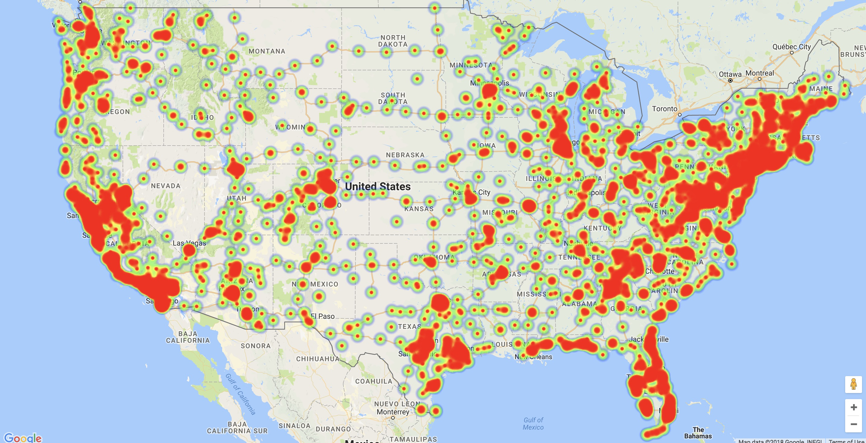
\includegraphics[width=15cm]{img/hotus.png}\\
		\caption{Distribution of Tesla Charging Station in the U.S.}\label{Figure1}
	\end{figure}

\begin{figure}[htbp]
	\centering
	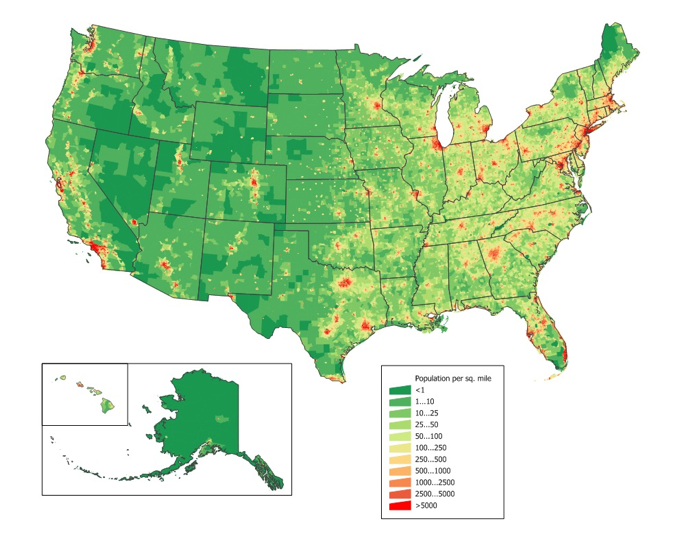
\includegraphics[width=15cm]{img/popus.png}\\
		\caption{Distribution of Population in the U.S.}
	\label{Figure2}
\end{figure}

We set the first formula based on the number of charging stations in the United States equal to the sum of the number of charging stations in each place: \begin{equation}
N_S = k_V*V_s
\end{equation}. We then contrast the two figures mentioned above and found two rules: 
\par
1. The distribution of charging stations is consistent with the degree of population density, and the heat is dispersed in similar areas. 
\par
2. In the less densely populated areas, if there is a charging station, only one situation arises where there is an expressway in the area, in other words, the road network. 
\par 
From this we can conclude that the number of vehicles and the number of charging stations depends on the population density and the distribution of the road network. As a result, we introduce the second formula:
\begin{equation}
V_S=k_P*P+k_R*R
\end{equation}


\par
We think that the number of charge stations and the power they provide needs to meet the charging needs of electric vehicles in each small area, so we derive the third formula:
\begin{equation}
N_U = \sum_{S}N_S 
\end{equation}
These serve as the data and theoretical foundation for our next grey prediction model and scale model.
		\subsubsection{Quantity of Charging Stations in All-electric USA}
		To estimate if Tesla is on track to allow a complete switch to all-electric in the US, we decide to determine if the variation trend of the number of Tesla electric vehicles could reach a certain level in the future to replace other types of vehicles.
		\par
We address the problem of predicting the number of electric vehicles through the grey prediction on account of a few data of the quantity of sale of Tesla electric vehicles. Using historical data(from the third quarter in 2012 to the fourth quarter in 2017) from Tesla, we determine the initial time periods for our prediction.
\begin{figure}[htbp]
	\centering
	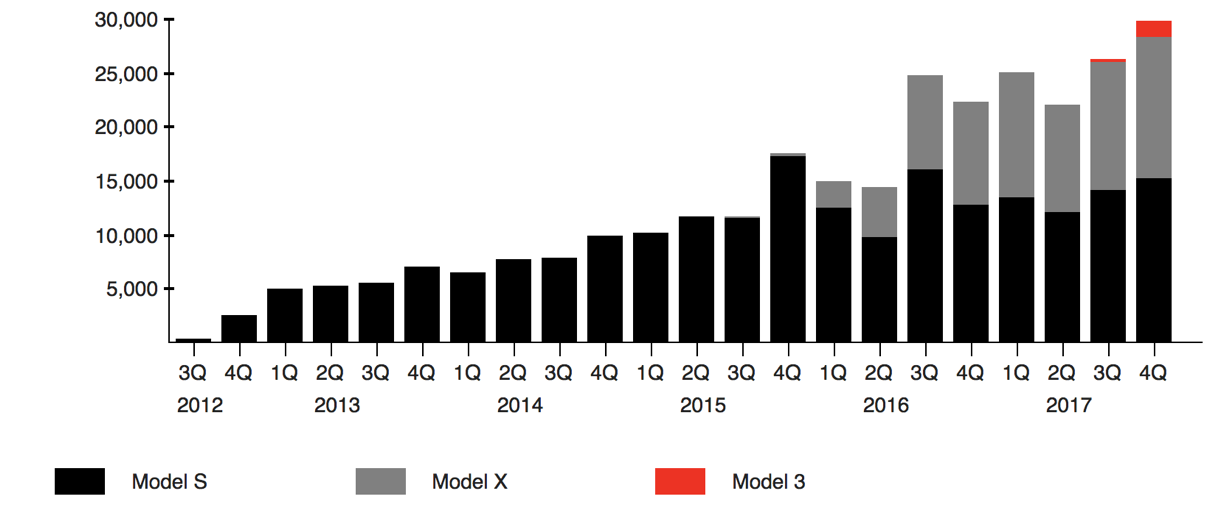
\includegraphics[width=15cm]{img/tsl.png}\\
	\caption{Tesla electric vehicle quarterly sales volume.}
	\label{Figure3}
\end{figure}
		\paragraph{Grey Prediction of Tesla Charging Stations Quantity:}
		The algorithm of grey prediction is described as follow:
		\par
		Assume $X^{(1)}={X^{(1)}(1),X^{(1)}(2),...,X^{(1)}(n)}$  is the cumulative sum of observed time series of the sales volume for the quarters.
		GM(1,1) model is defined by differential equation, $${{d{x^{(1)}}(k)} \over {dk}} + a{x^1}(k) = b$$ where $${[a,b]^T} = {({B^T}B)^{ - 1}}{B^T}{X_n}$$
		Fitting model to the data in the diagram, we get the red curve in Figure4.
		\begin{figure}[htbp]
			\centering
			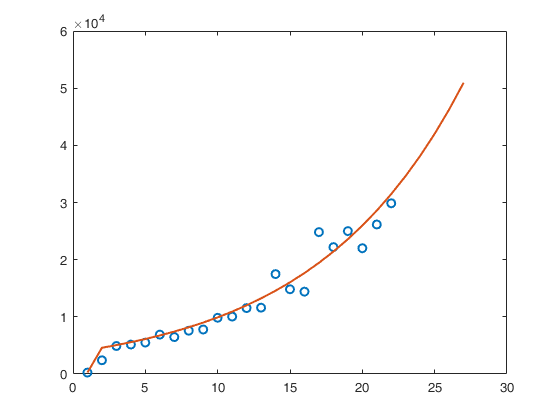
\includegraphics[width=10cm]{img/greyPredict.png}\\
			\caption{Gray Predict Model of Tesla  Charging Stations Quantity}
			\label{Figure4}
		\end{figure}
				We elicit a conclusion from Figure 4 that the number of electric vehicles increases exponentially from present to future which corresponds to our initial estimation as we define electric vehicles as a emerging industry that is analogous to the initial phase in the mathematic model of biological population growth.
				\par
				Then we use grey analysis which comes to a clear set of statements about system solutions.
				 At one extreme, no solution(or little information) can be defined or collected for a system with no information. At the other extreme, a system with perfect information has a unique solution. In the middle, grey systems will give a variety of available solutions. 
				 \par
				 Grey analysis does not attempt to find the best solution, but it does provide techniques for determining a good solution, an appropriate solution for real-world problems.[1]
				 
				 The grey analysis is divided into four phases. 
				 \begin{enumerate}[1.]
				 	\item We determine the number of the sales of Tesla electric vehicles that we have obtained as the reference sequence(generating sequence) $Y={Y(k) | k = 1,2,Λ,n}$,  the quantitative prediction as the comparison sequence(subsequence) $Xi={Xi(k) | k = 1,2,...,n},i = 1,2,...,m$. 
				 	\item The data in each factor column must be generally non-dimensional treatment in order to avoid the inconvenience brought by comparing data from different dimensions in the system) Thirdly, we calculate the correlation coefficient between x0 (k) and xi (k).
				 	\item We calculate the degree of correlation on account of the correlation coefficient is the correlation degree between the series and the reference series in between every time intervals (i.e, the points in the curve), it has more than one number, and the information is too scattered to facilitate the comparison.
				 	\item Making the correlation coefficient instantaneously (that is, the points in the curve) into one value to find the average value as the quantification of the correlation between the comparison series and the reference series. 
				 \end{enumerate}
			 We calculate that the value of r equals 0.8542 which means that our model predicts  is more consistent with practice.

		\paragraph{Logistic Growth  of Total Vehicles  Quantity}
		In the very beginning, we assume the maximum number of the U.S. cars is 300 million to approximate and to simplify the problem mainly because, in recent years, the number of the U.S. automobiles has grown unpleasantly, even with negative growth (shown in figure 5), and then combined with population restrictions, we estimated the saturation value of vehicles in the US is 300 million. Next, we use the logistic model to fit the total number of cars in the United States simply because theoretically, the model is a differential model that reflects finite growth, i.e, the growth of a variable in a system with an upper limit of growth and just as vehicles as a tool for people to travel, its demand is limited by the total population, so its growth has a ceiling. Additionally, according to figure 5, the number of registered vehicles in the United States from 1990 to 2017 also presented a form of logistic growth which supports our computing method.

		\begin{figure}[htbp]
	\centering
	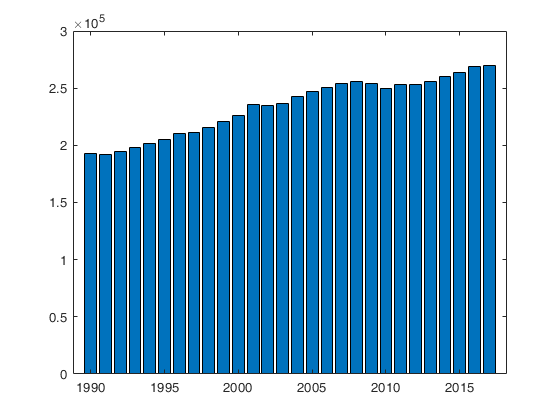
\includegraphics[width=10cm]{img/logistic.png}\\
	\caption{Logistic Growth  of Total Vehicles  Quantity}
	\label{Figure5}
\end{figure}
		\par
For the parameter x, starting from 1990, let x = 0, 1, 2, ..., 27 (i = 1990, 1991, ..., 2017). Then we obtain the regression equation:ans = $\frac{M}{{\mathrm{e}}^{-M\,\left(C+r\,t\right)}+1}$
To solve the differential equations in our model, we use MATLAB on the linearized equations(4)to find the result in figure and testify the regression coefficient and find it to be 0.9641, which is very close to 1, so the model can be used reliably to predict the total number of cars in the United States.
\begin{equation}
\ln ({\raise0.7ex\hbox{${{t \over M}}$} \!\mathord{\left/
		{\vphantom {{{t \over M}} {1 - {t \over M}}}}\right.\kern-\nulldelimiterspace}
	\!\lower0.7ex\hbox{${1 - {t \over M}}$}})
\end{equation}
		\paragraph{The Conclusion}
		After that, we combined two diagrams (figure6) to find the intersection which indicates the time of the all-electric society and the quantity of all-electric vehicles at that time.
		\par
As we mentioned above, Tesla is operating 892 super chargers and 3048 destination chargers currently, where as the number for current BEV(battery electric vehicle) is 286662. According to the result mentioned above, the prediction of BEV in all-electric society(future) equals 2.88e+8, we caculate the proportionality coefficient equals 1004.7, which is the quotient of the predict BEV number in all-electric society to current BEV number.
 \begin{figure}[htbp]
 	\centering
 	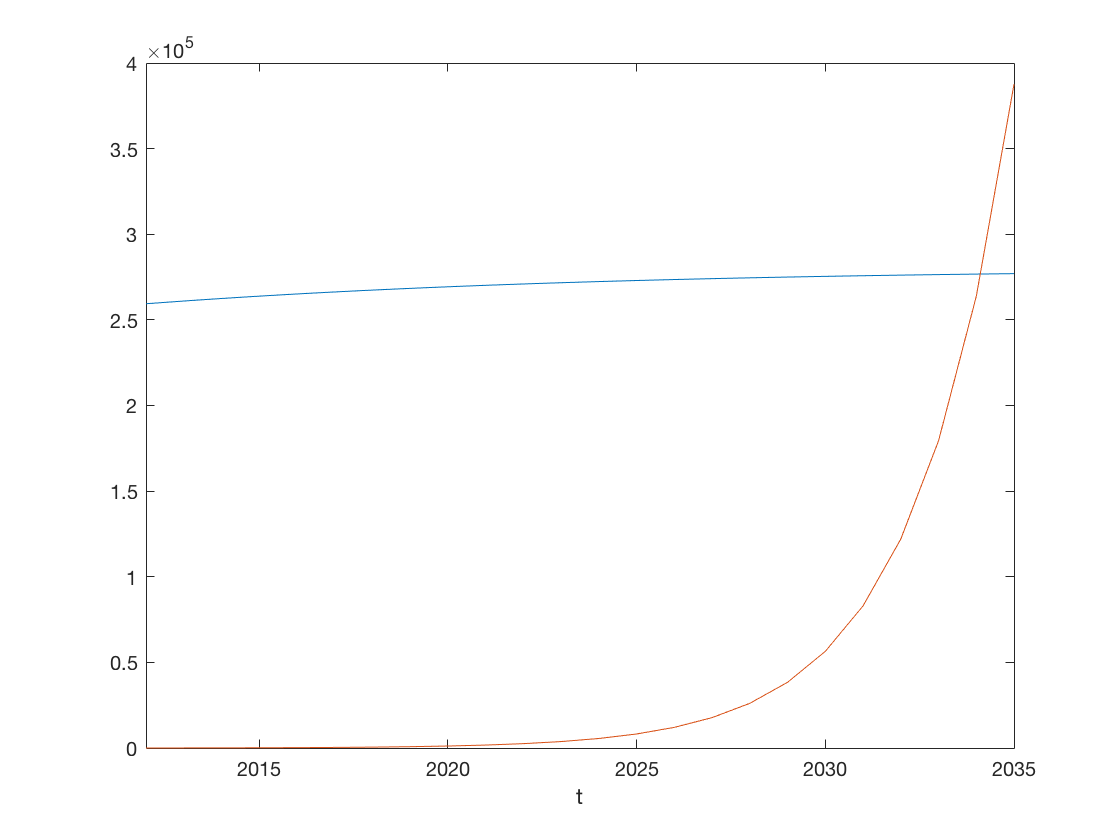
\includegraphics[width=10cm]{img/uspredict.png}\\
 	\caption{Combining Two Figures}
 	\label{Figure6}
 \end{figure}

\par

 
The proportionality coefficient can be more comprehensive because we believe the current distribution of electric vehicles is already representative which leads to an assumption that the distribution of electric vehicles is mainly related to the population, the efforts of local governments in implementing environmental protection policies, the length of road transport and traffic conditions, etc., but not related to the specific number of electric vehicles. Therefore, when the number of electric vehicles increases, the distribution (that is, the relative proportion of each area) will remain the same. The number of charge stations is to meet the charging demand in the area, so the distribution of charge stations is also unchanged. We successfully calculate the number for super chargers and destination chargers are 896164 and 3062227, respectively.
	\subsection{In Small-scale}
	Moreover, because the Large-scale Charging Stations Quantity and Distribution Model lacks flexibility, we tend to build a model that works for small regions.
Assume we divide area A into N blocks, annotated as $r_i$ sequentially. Under the hypothesis that the zero commuting time between each block and the automatic selection of the shortest route for users as mentioned above, we choose to view each block as a node abstractly. 
\par
Additionally, we use lines that connect nodes to represent the route. Each line will be given a value $T_i$, j whereas denotes the time required to travel from $r_i$ node/block to $r_j$ node/block for charging. Then, we first construct a NxN matrix A which is composed of $T_{i,j}$ to be further simplified. We define T as the longest time users are willing to spend to travel for charging. If $T_i$ is greater than 0, a value of 1 will be assigned, otherwise 0 will be assigned vise versa.(if $T_{i,j}$ is smaller than 0). As a result, matrix A will be transformed into the format of E. In other words, in between N nodes, if $E_{i,j}$ equals 1, then there is one line connected between $r_i$ and $r_j$; if $E_i$ equals 0, then $r_i$ and $r_j$ are boundlessly connected to form an abstract graph.

Using the Algorithm 1 in appendix, we can determine a division of ri as $R \{R1, R2 ... Rm\}$. For any divided Ri we can determine that it contains $\{r_{i,1}, r_{i,2} ... r_{i,n}\}$ nodes. $\sum_{i}^{n}\sum_{j}^{n}b_{i,j}$) is the total demand for charge stations at $R_i$ which should not be exceeding the sum of $c_{i,j}$. The cost causing by the lack of charging stations is measured by a linear 
Aim at determining the minimum value of $\sum_{i}^{n}\sum_{j}^{n}d_i*c_{i,j}+\sum_{i}^{n}\sum_{j}^{n}e_{i,j}*k_{i,j}$
constraint condition:$\sum_{i}^{n}\sum_{j}^{n}d_{i,j} >= \sum_{i}^{n}\sum_{j}^{n}{b_{i,j}}$
By using linear programming to solve each $d_{i,j}$, resulting in the distribution of charge stations.

\subsection{Apply to town and country planning}
	Here we build small-scale charge stations quantity and distribution model to solve the city, suburbs, rural distribution of charge stations.
In the very beginning, our idea was to divide each area into different squares for nesting, and also to represent each charge station with a small square that was cut out as the graph 1. Such a square nested idea has some advantages, for example
\begin{enumerate}[1.]
\item Use this kind of nesting, it makes the process of solving the distribution problem more convenient because the representation of the graphic is a square, which is relatively common. 
\item A small number of nodes and well-distributed, the discussion is less difficult. 
\item  The square easily covers the entire area without omissions. 
\end{enumerate}
Nevertheless, it also has some drawbacks at the same time: 
\begin{enumerate}[1.]
\item The square cannot reflect the shape of the area that the charge station can radiate because the area irradiated by common sense is generally indicated by a circle. 
\item The method of "dividing and nesting with squares" is less similar to the actual situation.
\end{enumerate}
To overcome these challenges, we decide to combine and apply Chris Taller central place theory to our model. As shown in the graph (2), we improve it to look like a beehive, internally dividing the nodes with 54 congruent equilateral triangles. In this way, it has more advantages, and the model is more appropriate to the actual distribution of charge stations in cities, suburbs and villages while retaining the characteristics of "easy to cover and tiled specific areas." Nonetheless, we find that there are some difficulties as well. In this method of division, its number of nodes is too large to calculate which further makes the model more complex. 2. Triangle and radiation patterns still differ in many other perspectives. After further optimization, we introduce a model as shown in the graph (3), which divides the urban, suburban and rural areas into three-layer by red lines and combines the characteristics of the central place theory to make the division form more compact and more realistic. Meanwhile, the number of nodes is determined to be 21 when we center each block as a node the graph (4), the number is smaller and the hexagonal shape shares more common characteristics as the area irradiated by the charge station.

 \begin{figure}[htbp]
	\centering
	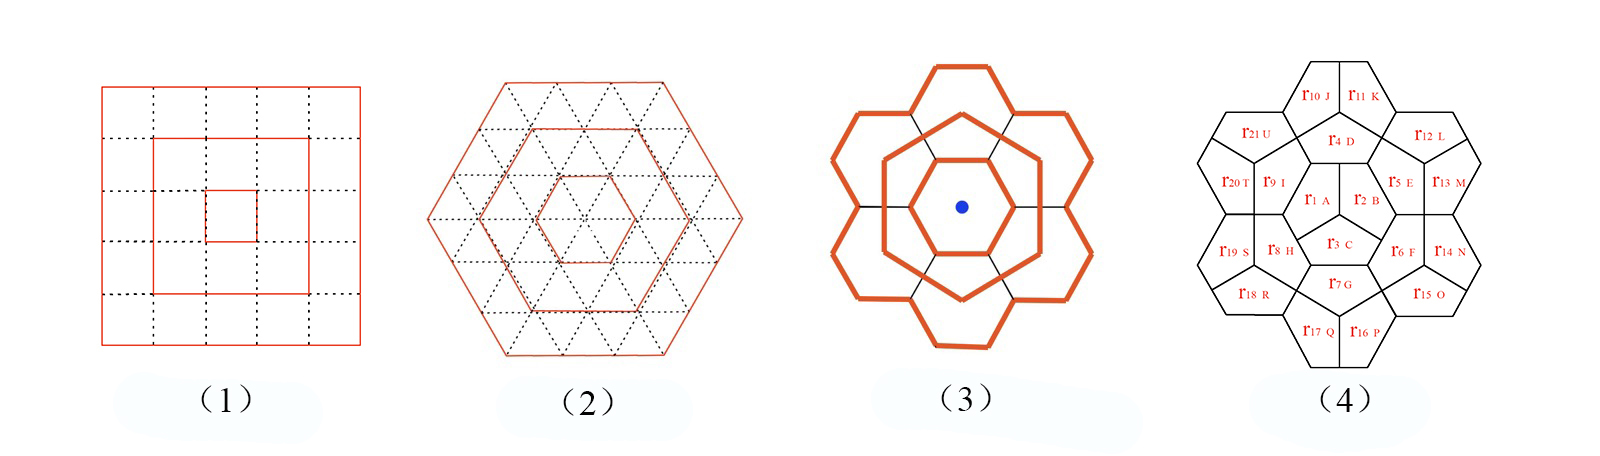
\includegraphics[width=15cm]{img/img710.jpg}\\
\end{figure}

After determining the model design, we then determine N = 21, set at 21 nodes $r_1, r_2, ..., r_{21}$ (ie, 21 regions), the value of Ti depends on two factors: 
\begin{enumerate}[1.]
 \item $p_{i,j}$The distance between $r_i$ and $r_j$, we can see the value of $p_{i,j}$ in this model only contains a,${a^{1/3}}$,$\sqrt 3 a/2$ (geometry (5))
 \item The degree of congestion $\lambda_{i,j}$ is determined by which of $r_i$ or $r_j$ in the cities, suburbs and villages.
We assume the following sheet indicates the ranges for blocks from urban, $c_{i,j}$ suburban $k_{i,j}$ and rural areas($b_{i,j}$). 
 \begin{figure}[htbp]
	\centering
	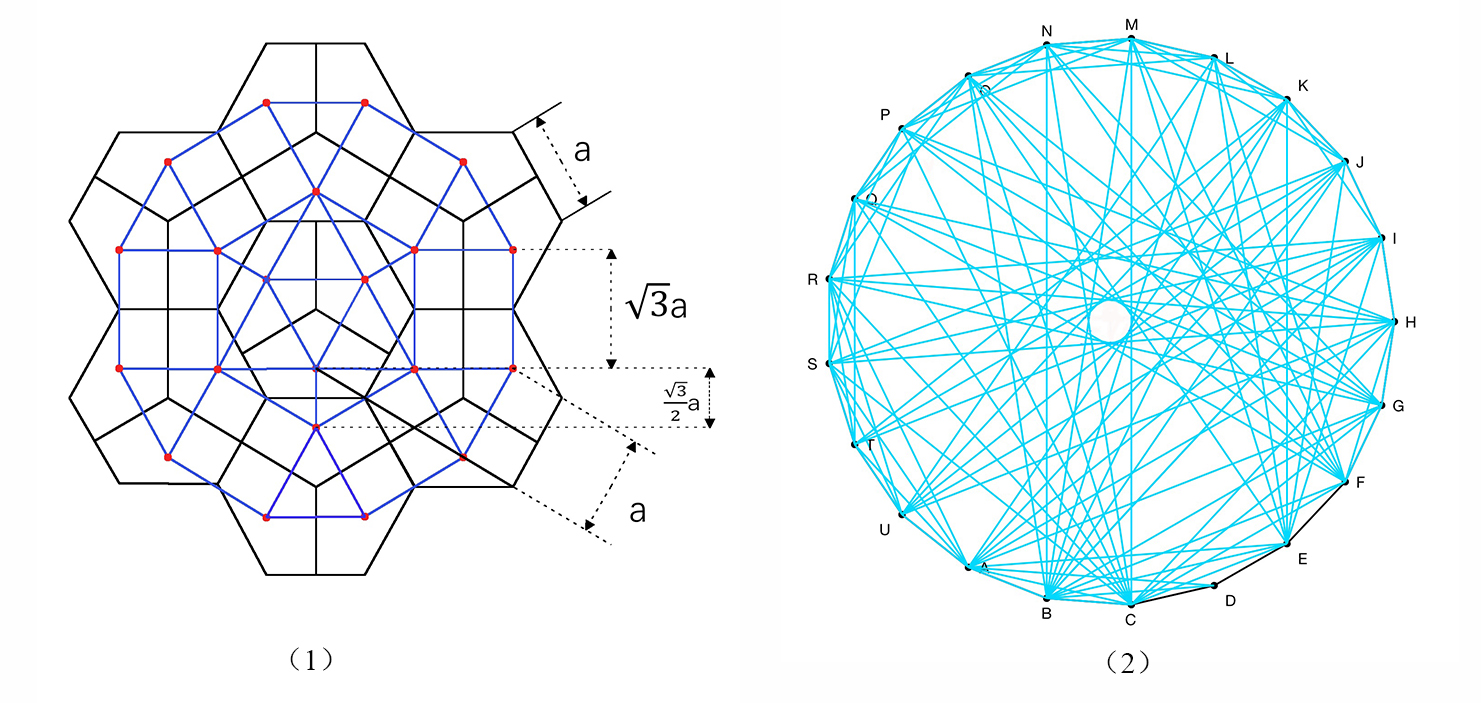
\includegraphics[width=12cm]{img/img12.jpg}\\
\end{figure}
In order to facilitate the calculation process, we assume the three types of lines to correspondingly represent routes that are 10km, 17km and 20km long. With the car speed of 60 km/h, $λ_{i,j}$ ranges 2.25 (1.5*1.5) in between urban areas, 1.8(1.5*1.2) in between urban and suburban areas , 1.44(1.2*1.2) in between suburban areas, 1.2(1.2*1) in between suburban and rural areas and 1(1*1) in between rural areas.
$T_{i,j}$=$p_{i,j}$/60* $λ_{i,j}$
we can list the matrix of $T_{i,j}$ as shown in the one table. Using the simplifying method introduced above, we can get matrix E  and to plot an abstract the graph6. Then divide again based on the algorithm 1  to result in four subgroups with different color codings as indicated in the graph 7.
\par
After applying the idea of linear programming using LINGO for calculations, we concluded that the percentages of electric cars charging stations are 57\%, 29\% and 14\% for urban, suburban and rural areas respectively.
\end{enumerate}
\section{Practical Application of The Model in Ireland}
When we consider the optimal number and distribution of charging stations if Ireland could migrate all its personal passenger vehicles to all-electric vehicles instantaneously, we combine this estimation with the proportionality coefficient mentioned in the US. We derive the proportion in Ireland from the ratio of electric vehicles and charging stations in the United States. As we assume that the distribution of electric vehicles is mainly related to the population, the efforts of local governments in implementing environmental protection policies, the length of road transport and traffic conditions, etc., but not related to the specific number of electric vehicles, we can define the formula: The total number of vehicles in Ireland/The total number of electric vehicles in the US*The number of super charges in the US. Similarly, the number of destination charges applies to the formula too. We substitute the data that needed(The total number of vehicles in Ireland searched from [2] etc.) and calculate the result 39288.

We collect the daily average number of vehicles recorded at 295 monitoring sites on the Irish Expressway from 2014 to February 2018. Then take their average, calculate AADT.Among these 295 monitoring sites, some of the monitoring sites are on the same road, and we can obtain 84 integrated data after merging the monitoring points on the same road. Then take the average of the  longitude and latitude on specific road and combine it and AADT to obtain the traffic flow. The result is shown in the thermogram(figure 14) that we can observe the distribution and placement of charging stations clearly. As you can see, the four metropolitan cities centered in Dublin, Athlone, Cork and Kilkenny are the four largest circled areas on the thermogram and because the thermogram matches the proportional model, we suppose the most crucial factor that can be derived from our model and practice is traffic flow.
 \begin{figure}[htbp]
	\centering
	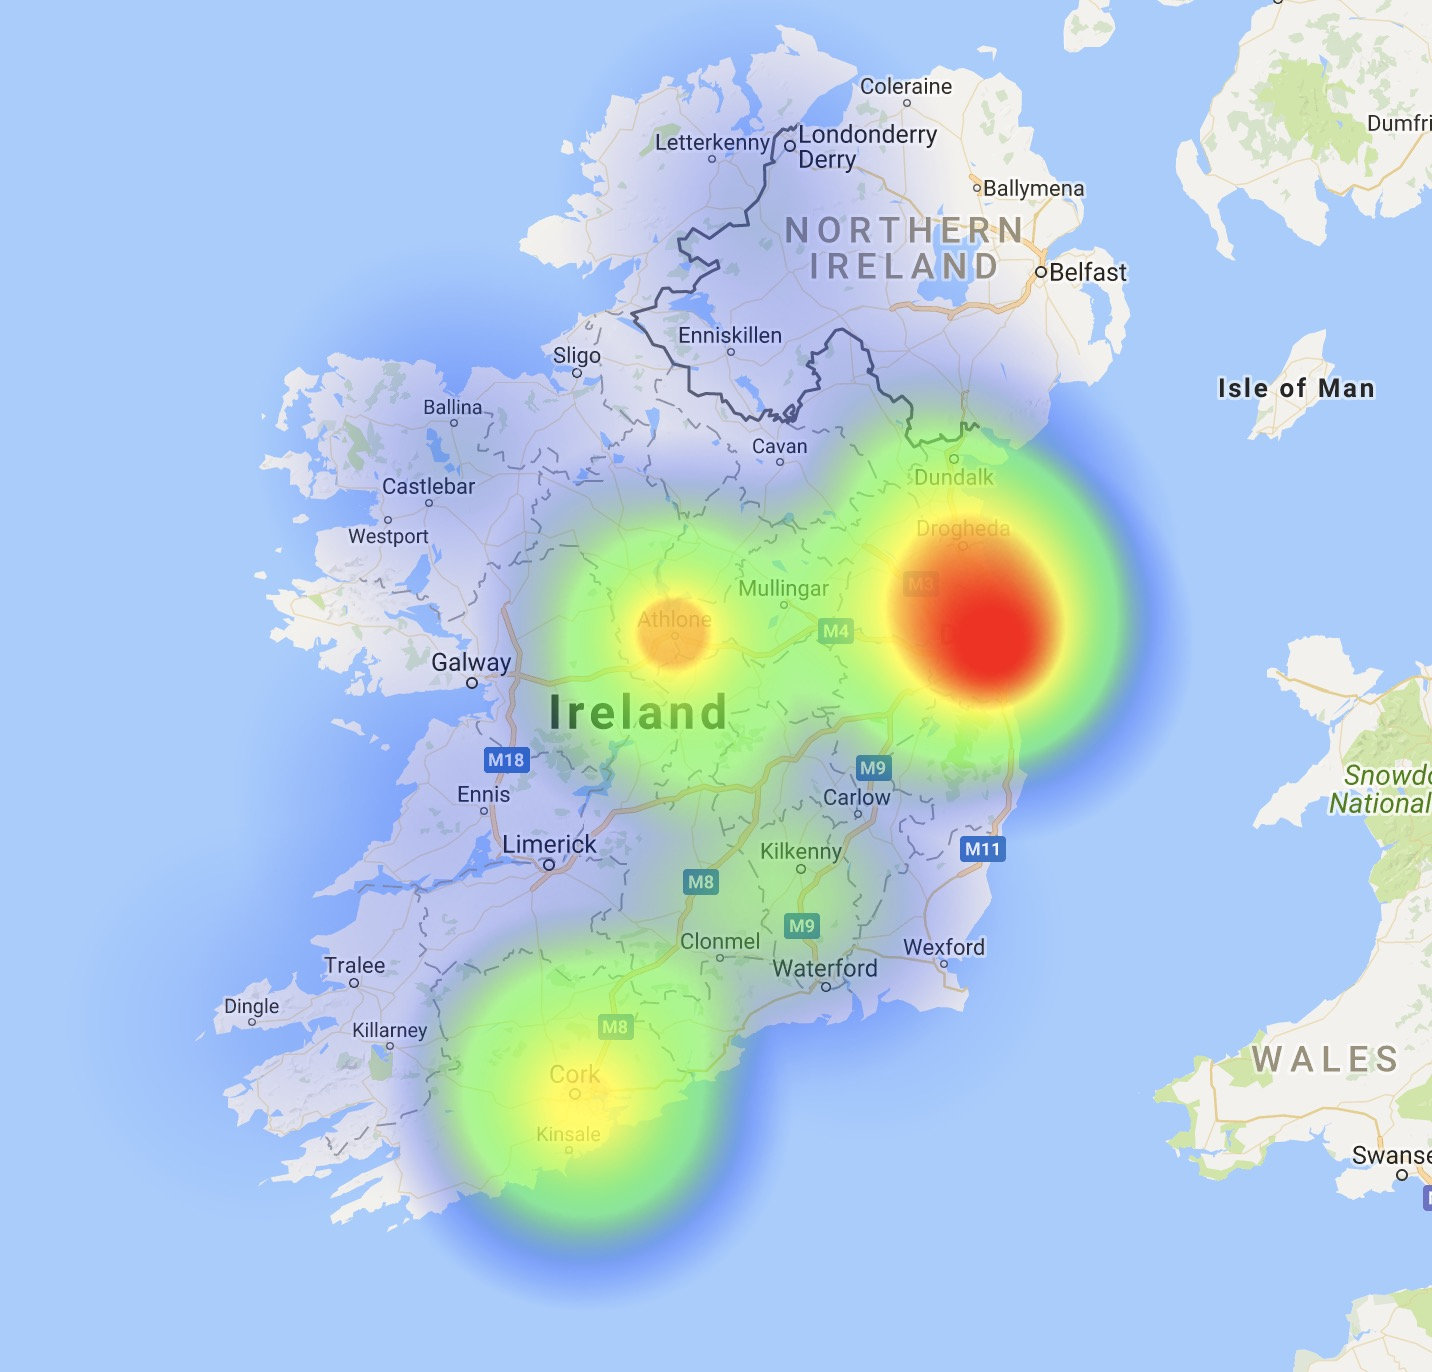
\includegraphics[width=10cm]{img/monheat.png}\\
	\caption{Traffic Hotmap in Ireland}
	\label{Figure7}
\end{figure}
\section{Multi-factor Cooperative Growth Model}

In the discussion above, we imaged a one-day transform to all-electric society. In reality electric vehicle industry in Ireland is now in the early development, we have to start with a little foundation. While the U.S have already installed a huge charging network chargers(3940 tesla charger station, comparing 22 in Ireland), it is no longer appropriate to reuse the Large-scale and Small-scale Charge Stations Quantity and Distribution Models mentioned above because we think we should focus on "how to invest" and give our proposal to those countries which lack practical and investment experience.  
\par
We construct Multi-factor Cooperative Growth Model. The model is inspired by biological mutualism, where each of the species population is influenced by that of the others. We notate the ratio between the number of charging stations and the number of electric cars as $NV_{ratio}$. When the ratio is extremely low, it will result in a dramatic decrease in electric-car users since both the time needed and money spent on charging become unreasonably high. On the contrary side, if the ratio is too high, numbers of charging stations will be idle or even get shutdown. At the same time, according to  theories from economics suggested, our market will adapt to changes in both internal and external (many) factors to reach the ideal market equilibrium. For example, if the ratio is low, suppliers will seek this opportunity to construct more charging stations to maximize their revenues. Conversely, if the ratio is high, buyers will realize how convenience it is for charging which will probably further prioritize electric cars as their their preference. We can use the following equation to illustrate this market equilibrium relationship: 
\par

After that , we add up the influence with some other factors that're considered to have an affect on the growth of the model and draw a conclusion as the formula below.
Influence factors:
\begin{enumerate}[1.]
	\item $R$: Urban-rural development balance index(To measure the balance between urban and rural development.)
	\item $a_1, b_3$: Government investment effective index(To measure how total government investment and the proportion of government's investment in electric vehicles and charge stations impact on the result after the investment.)
	\item $a_3$: People's acceptance of electric vehicles index(To measure how willing people are to accept the mode of electric vehicles using.)
	\item $I_t$: The duration of government investment index(To measure the duration of government initial investment.)
	\item $M_s$: The saturation index of vehicles.(To measure the saturation value of vehicles in a specific country.)
\end{enumerate}

\par

\section{Sensitivity Analysis}
Now we will discuss the sensitivity of each factor to the model result.
Among these the factors $NV_{ratio}$, the saturation index of vehicles and urban-rural development balance index index is decided by the situation of national population and geography. $NV_{ratio}$, people's acceptance of electric vehicles index and the duration of government investment index are three key variables that can be adjusted by policymakers, which will be discussed below.
\par
However, our first work is to decide a proper numeric value of the government investment promotion index. We referred to the investment data and its effect of U.K., the neighboring country of Ireland: The British government decides to achieve an all-electric society using 20 years. As an important part of the budget, the current British government has allocated funds for plug-in hybrid projects, which have lowered the selling price of such vehicles by 4,500 (about 5,995 U.S. dollars) and will be invested by the British government by 2020 for 100 million pounds (about 130 million US dollars).  In addition, more importantly, the British government is developing a regulatory structure designed to invest 400 million pounds (about 530 million U.S. dollars) for the Charging Investment Infrastructure Fund, of which 200 million pounds \$270 million) from the private sector to promote the charging infrastructure. After implementing such an investment policy, the number of electric vehicles in Britain increased by 7,000 as the total number of connectors has increased from just over 11,000 in February 2017 to more than 14,000 by Jan 2018.[4][5] Basing on these data, we estimated the government investment promotion for England, then we find the contrast between Ireland and England and decided the model parameter for Ireland.
\par
Using MATLAB, we got the result of the model. Initially, we set $NV_{ratio}$ at 0.8, and government enact a 5 years investment to the electric car industry. We got the following figure. the x-axis is the month from now, the y-axis is the amount of vehicle or charger station. The unit of the y-axis is one thousand. The green curve shows the amount of the electric cars and the purple curve shows the amount of the charging station. Four parallel lines from bottom to top of the X-axis indicate 10\%, 30\%, 50\% and saturation line, respectively.As we can see, with this investment, the amout of cars failed to reach its saturation value(3000 thousand) in 20 years. 
 \begin{figure}[htbp]
	\centering
	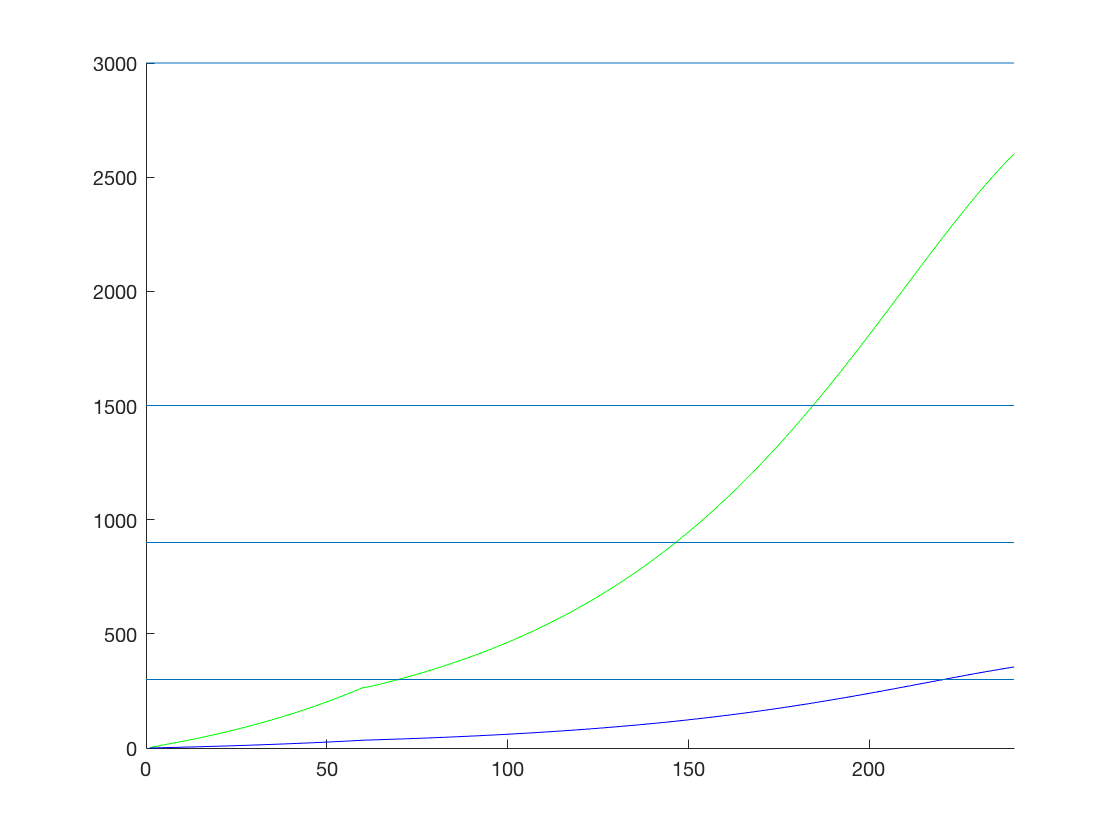
\includegraphics[width=5cm]{img/ireland08.png}\\
	\caption{$NV_{ratio}$ =0.8}
	\label{Figure7}
\end{figure}
\subsection{Discussion of $NV_ratio$ change}
To discuss the effect of different policies on the growth. At first, we lower the $NV_{ratio}$ to 0.3,  which means a prefer investment tendency to the vehicles. In this way, the number of electric cars reached its saturation point in 20 years. However, observing the $NV_{ratio}$, a considerable oscillation is showed in the early stage, indicating the charging stations could not satisfy the fast-growing electric cars. What's worse, it spends around five years to achieve the ideal proportion and stay at the equilibrium point, which brings a bad user experience for early adopters. In constract, when $NV_{ratio}$ is 0.8, the oscillation is eliminated and the ideal proportion is achieved in the very early one year. To conclude, lower $NV_{ratio}$ helps accelerating the growth of electric vehicles while higher $NV_{ratio}$ helps improve the experience of initial users. However, They are not the main factors that affect the result of the model. It should be noted that there's a drop-down point when the government stopped investing after the fifth year.
\begin{figure}[htbp]
	\centering
	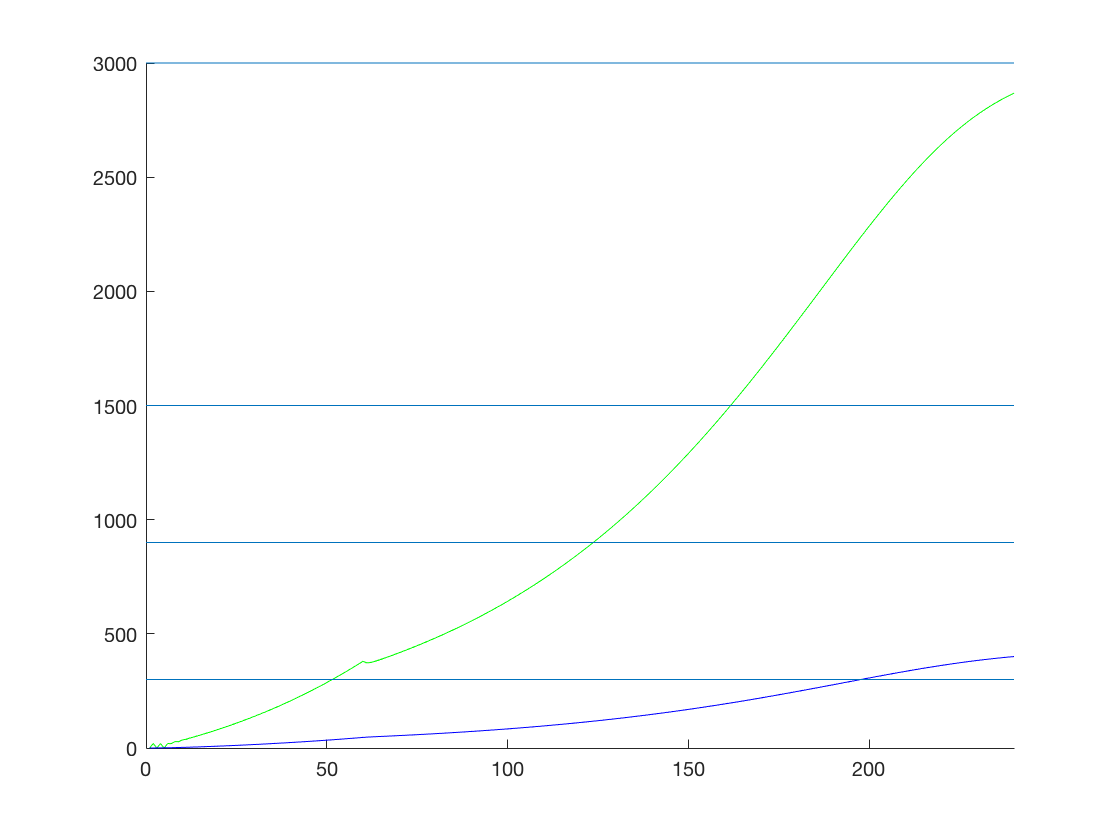
\includegraphics[width=5cm]{img/ireland02.png}\\
	\caption{$NV_{ratio}$ =0.2}
	\label{Figure7}
\end{figure}
\begin{figure}[htbp]
	\centering
	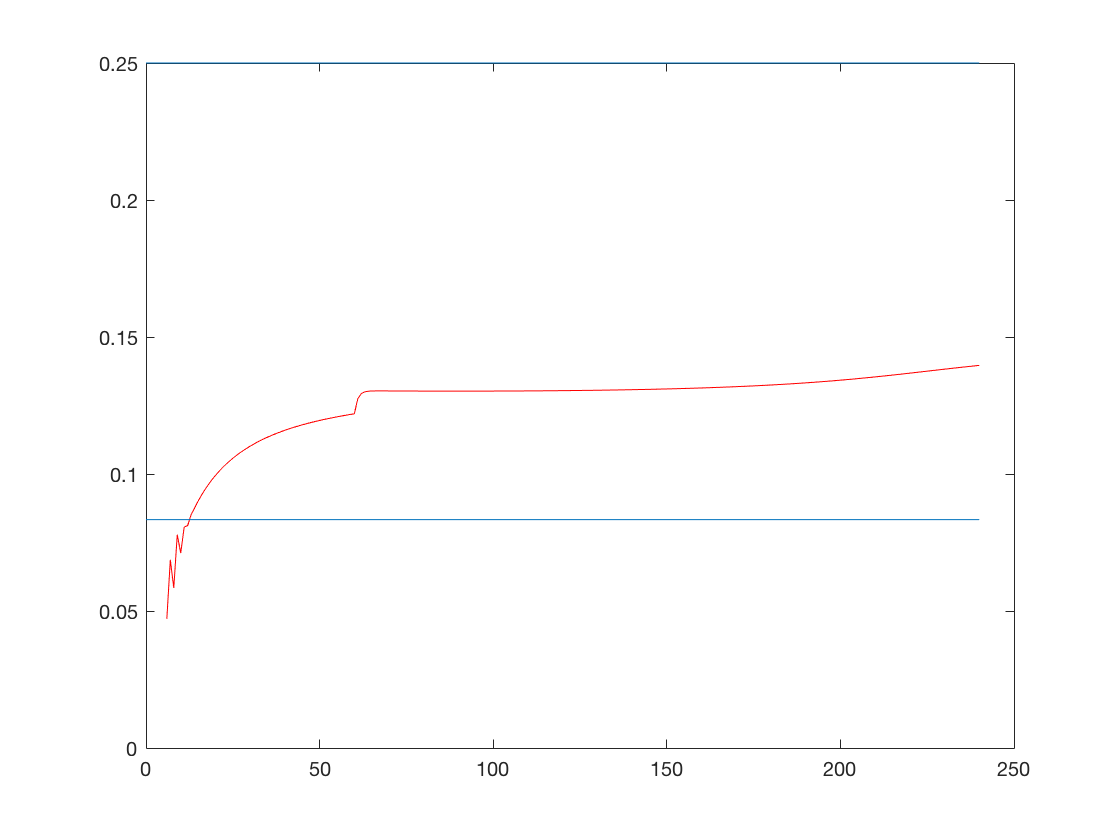
\includegraphics[width=5cm]{img/ireland02ver.png}\\
	\caption{$NV_{ratio}$ =0.2}
	\label{Figure7}
\end{figure}
\subsection{Discussion of $I_t$ change}
Secondly, we keep $NV_{ratio}$ at 0.8 and adjust the duration of government investment to 10 years,  the dropdown phenomenon is disappeared. This suggests that the market already is able to resist fluctuations of  external factors and healthy development. As a result, The goal of all-electric society is basically realized in 20 years. Therefore, We propose that the government should maintain the stability of investment policy until this market is mature.
\begin{figure}[htbp]
	\centering
	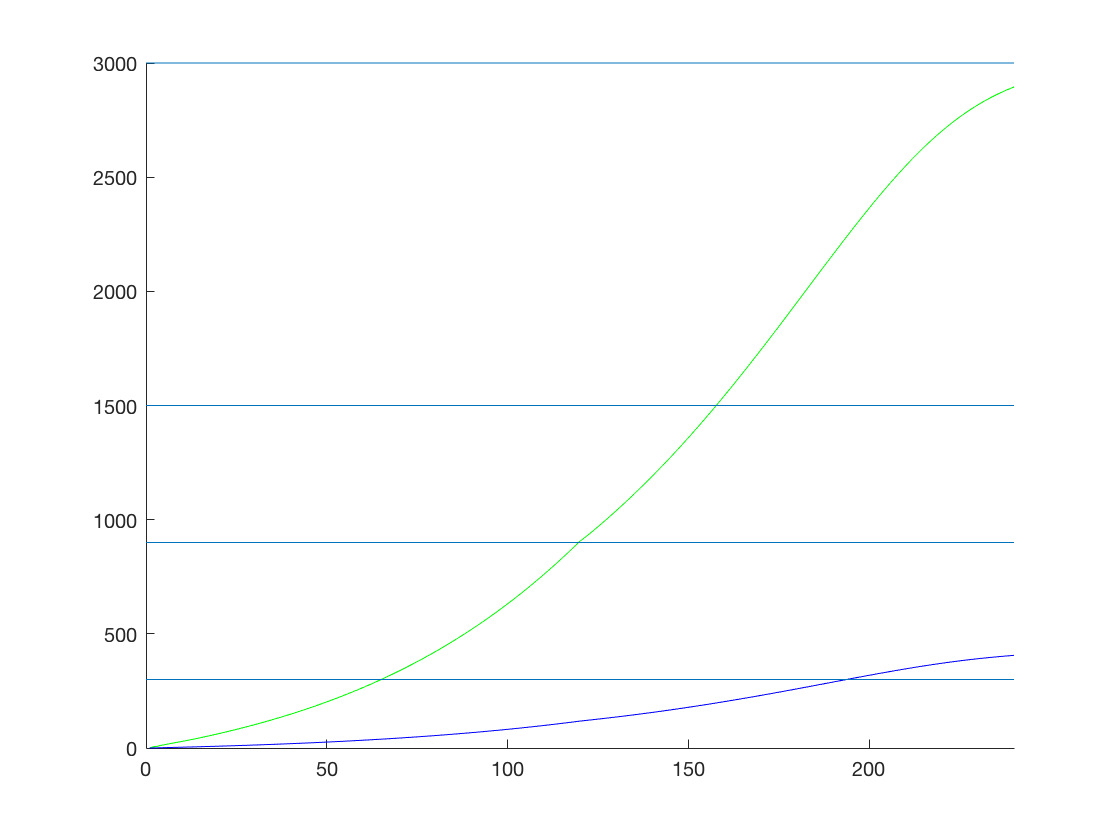
\includegraphics[width=5cm]{img/ireland10year.png}\\
	\caption{$I_t$ doubled}
	\label{Figure7}
\end{figure}
\subsection{Discussion of $a_3$ change}
The last, We considered the change in people's acceptance of electric vehicles, when we double this factor, the growth curve changed dramatically, In just 12 years, an all-electric society has been achieved. In reality, the acceptance of electric cars is unlikely to grow so fast, However, the effective publicity of the electric car performed by government and the media can help promote in a certain extent.
\begin{figure}[htbp]
	\centering
	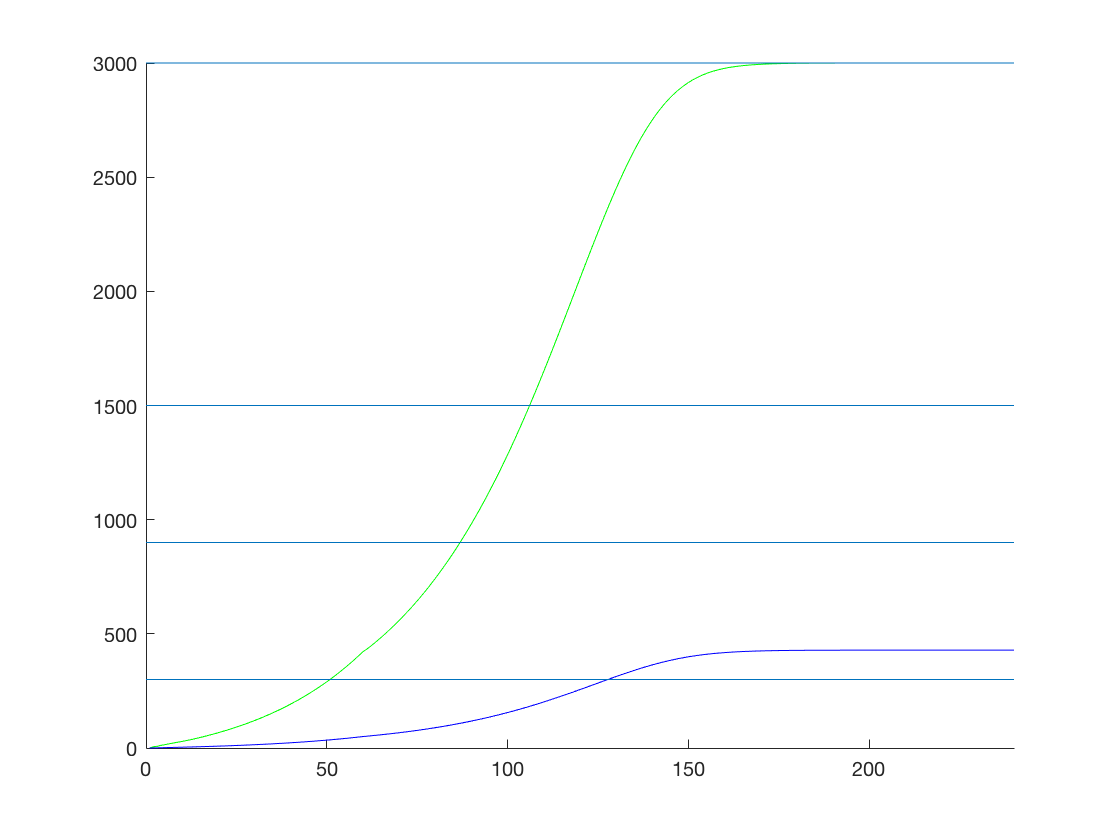
\includegraphics[width=5cm]{img/ireland014.png}\\
	\caption{$a_3$ doubled}
	\label{Figure7}
\end{figure}
\section{Scalability}
In order to validate the model's scalability, we select China especially as the object of our study that has a huge difference from ​​Ireland in the area of the country.(Also for each country, we estimate the optimal $NV_{ratio}$ and the investment duration) China has a population of 1.4 billion. Since China has a developed public transportation system, Chinese people prefer to share a car in a family, There is a clear difference between China and the United States at this point. Therefore, we estimate that China's automobile saturation and the outcome is about 450 million. By investigating China's average monthly auto sales volume, we set the Chinese government's investment efficiency coefficient to reach 17 times that of Ireland. In this case, we found that the model can still operate normally. Since China has a low urban coverage and a wide rural area, China should pay more attention to the balanced development of charging stations and electric vehicles in urban and rural areas.
\begin{figure}[htbp]
	\centering
	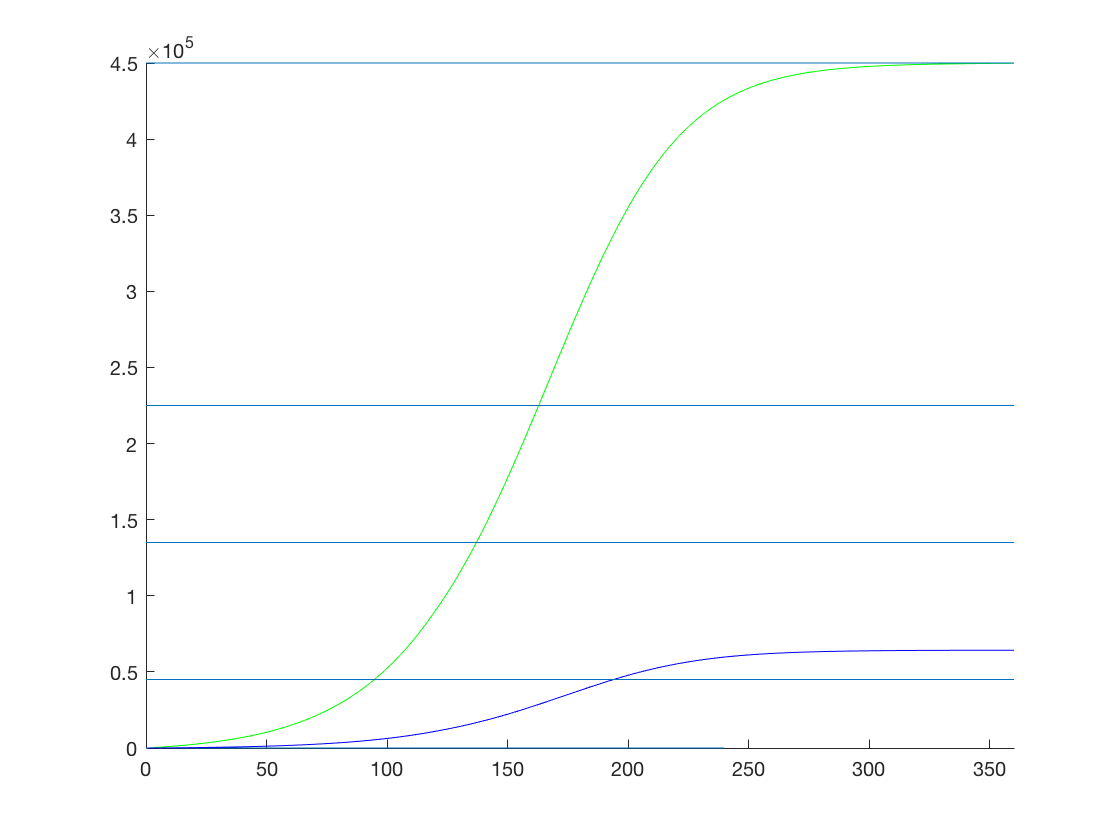
\includegraphics[width=5cm]{img/china.png}\\
	\caption{$Applied to China$}
	\label{Figure7}
\end{figure}
\section{Evaluation of the Model}
	\subsection{Large-scale Charge Stations Quantity and Distribution Model}
	Strengths: \par
	1.Establish the model by observing the real world which makes it own a high fidelity to reflect the general rules of the number and distribution of charging stations.\par
	2.The calculation is small, but it can well reflect the problem of distribution of charging stations in a large area which is difficult to solve by using graph theory modeling.\par
	Weaknesses:\par
	1.When using it for long-term forecasts, because of the unpredictable changes to the traffic volume, population and road network in a wide range of regions are so complex that we can only fit future data based on what is currently available.Overall the model lacks flexibility.\par
	2.This model only considers the charging needs of electric vehicles and does not consider the optimization of distribution and investment costs.\par
	3.In the process of using grey prediction, we find a little historical data. Although the obtained fitting is almost perfect, the variance of the residual error tends to increase when the residuals are tested, which will increase as time goes on, leading to prediction that is not entirely accurate.
	\subsection{Small-scale Charge Stations Quantity and Distribution Model}
	Strengths:
	1.The model can solve the problem that choosing the site where the users and vendors pay the least cost in the small area with known traffic nodes and road distribution, and achieve a win-win situation for users and manufacturers.
	\par
	2.The model abstracts each area as a node, abstracting the road as a hexagon edge, giving coordinates and values ​​of specific locations and applying it to actual urban planning.
	\par
	Weaknesses:
	\par
	1.The model involves superabundant nodes, the calculation is too large and it is difficult to apply in a large-scale situation.
	\par
	2.We did not consider scrapped electric vehicles.
	
%	\subsection{The Urban - rural Area Division Model Based on Improved Central Place Theory}
%	Weaknesses:
%	\par
%	1.The model assumes that the time it takes for the BEVs to charge themselves in the same area is zero, but it is not reasonable in reality because it does not take the impact of the terrain into account.
%	Combined the Small-scale Charge Stations Quantity and Distribution Model and The Urban - rural Area Division Model Based on Improved Central Place Theory, they can make up for each other's deficiencies and learn from each other's advantages.
	
	\subsection{Multi-factor Cooperative Growth Model}
	Strengths:
	\par
	1.The creative combination of the characteristics of the symbiotic model in biology reflects the complex feature of the system in which the number of charging stations and electric vehicles influences each other.
	\par
	2.The model takes into account a variety of factors that make the model very flexible and scalable, so that it can be widely used in countries with very different geographies, population density distributions, and wealth distributions, thus making it possible to establish a classification system in different countries.
	\par
	Weaknesses:
	\par
	1.Since there are too many variables in the model, we use the data in England as the basis for confirming the parameters, but such a method may not be reliable.
\section{Influence of Exogenous Events}

	The technological world continues to change and is impacting transportation options such as car-share and ride-share services, self-driving cars, rapid battery-swap stations for electric cars, and even flying cars and a Hyperloop. Comment on how these technologies might impact our analyses of the increasing use of electric vehicles.
	\par
	Living in such a technology dependent world changes the ways and methods people approach certain things. For instance, transportation options such as car-share, rideshare have gained their public recognition and are becoming more and more popular from day to day. Technologies within the transportation sector not only alleviate traffic and environmental problems, but they also save time and money for its users.
	\par
	According to scientific researches, having too many cars requires extracting a huge amount of fuel gases while producing health-threatening poisonous gases at the same time. In fact, 93,500,000 barrels of fuel gases are consumed per day in the world. Moreover, each galloon has the ability to result in 798 pounds of heat-trapping emission. [7] As a result, the transportation sector has accounted to be one of the biggest contributors to the overall air pollution in the world. [8] Although we cannot change the pessimistic pollution numbers from the past, we can incorporate the newest services and technologies into our transportation systems to mitigate its negative consequences resulted from the past.
	\par
	Car-sharing and ride-sharing are the two most well-recognized service programs that help people to drive less. Bollore, a company which owns electric vehicle sharing plans, takes its initiative by launching car-sharing program in eight different cities across the world. [9]As indicated on Bollore’s official website, “The Group produces and sells electricity storage solutions for both mobile and stationary use, ranging from the production of electric vehicles and the creation of car-sharing systems to complete solutions to produce, store and distribute decentralized, clean and free electricity, via solar energy”. [10] Through the car-sharing program, fewer cars will be on the road which helps alleviate not only the air pollutions, but also traffic congestions. Intelligent Energy Europe has published a report about “The environmental impacts of Car-Sharing Use” which gathered many statistics and evidence to conclude that car-sharing use consumes a 25\% lower fuel on average. [11] Ride-share is another similar program provided mostly by university students. Instead of driving by yourself, people participate in an arrangement in which a passenger travels in a private vehicle driven by its owner, for free or for a fee, especially as arranged by means of a website or app. As the trend of car-sharing and ride-sharing programs becoming more popular under the assistance from the service technology, fewer cars will be demanded to be driven on roads.
	\par
	As our technologies have been constantly developing, many new forms of transportation have been introduced such as self-driving cars, rapid battery-swap stations for electric cars, flying cars and Hyperloop. According to The Independent newspaper, “driverless electric cars could cut air pollution to almost zero and make car parks obsolete within 10 years”. [12] Self-driving cars will not require any parking space since they will head off and carry out their next journey after dropping passengers off. As a result, governments can construct fewer transportation infrastructures but plant more trees on idle lands. Alternatively, more parks can be built on lands that were previously occupied as parking spaces. On the other side of the spectrum, cars without drivers require less gas compared to cars with human drivers. Statistics gathered by “Greener Ideal” suggested that “most gas is burned when driving at high speeds, braking, and re-accelerating excessively”, but “self-driving vehicles cut these factors out of their driving style” which results in less air pollution. [13]Another proposal of flying cars came from Kitty Hawk as an alternative solution to mitigate environmental consequences from driving. Sebastian Thurn, the C.E.O of Kitty Hawk, said: “Flying cars have flexible routes which do not require any roads at all” [14]. Similarly, Hyperloop is proposed as another innovative transportation method. Elon Musk, the C.E.O of SpaceX, viewed this technology as “incorporating reduced-pressure tubes in which pressurized capsules ride on air bearings driven by linear induction motors and air compressors”. [15] After the idea was proposed, many professionals have put hours of hard work and finally implemented different test systems across different companies such as Virgin and SpaceX. As the most recent data shown on Futurism’s official website, “Virgin Hyperloop Once announced its testing capsule has reached nearly 387 km/h, breaking the 355 km/h speed record set by Elon Musk’s Hyperloop in August”. [16]Although both the flying cars and Hyperloop require a large amount of financial support, they have been predicted to be “low-cost transportations on long run” since they produce nearly none or little pollutions.[17]
	\par
	Technologies within the transportation system also help people to save both their money and time. The Newsroom has conducted many researches to conclude that “the average cost of driving is $8469 annually, or $706 each month”, [18] let alone other financial products attached to driving such as car insurance. New technology-based services such as car-sharing and ride sharing allow passengers to pay less while providing the same privilege of flexible pick-up and drop-off times and locations as driving. Moreover, under the sharing systems, many people are splitting the pie of maintenance bills such as insurance or fuel charges of one vehicle when paying for their rides. Another advantage that electric cars have over fueled cars is that the bills for cars are relatively fixed. Fuel price fluctuates every day since it depends on many factors such as government policies or external environments. On the contrary, electric cars use electricity which its price is relatively stable compared to fuel price, as their power source. Although on a timely basis, road-dependent vehicles such as car-sharing, ride-sharing services and self-driving cars do not express as much difference as flying cars or Hyperloop have when compared to normal cars, they can still alleviate traffic problems on roads since fewer cars will be demanded to be driven on roads. Flying cars and Hyperloop are considered as extremely high-speed transportations once it is successfully launched to all public in the future. Some specialists also proposed the idea of introducing rapid battery-swap stations for electric cars to eliminate the time for charging, but the idea has not gained enough public interests or recognitions yet. As a result, Tesla postponed the initial launch date for further development.
	\par
	To conclude, varies technologies revolutionized the transportation sector by using renewable energies instead of natural resources, mitigating poisonous gas air emissions and saving money and time for its users simultaneously.
	\newpage
	Dear Sir,
	\par
	Upon hearing that the leaders of a wide range of countries are attending an international energy summit,  my fellow colleagues and I are honored to engage in clearly communicating our role and scope of engagement in the development of electric vehicles industry.  We have been working with painstaking efforts so as to do something for the world concern of plans to migrate personal transportation towards all-electric cars and we do have some outcome by researching day and night these days, which we hope can be of help in providing a suitable plan for electric vehicles and 
	charging stations construction for your country.
	\par
	Inspired by Large-scale Charge Stations Quantity and Distribution Model, we establish the model by observing the real world which makes it own a high fidelity to reflect the general rules of the number and distribution of charging stations. We firmly believe that when your country plans to do long-term planning for electric vehicles and charging stations, you should closely follow the population distribution and road network structures based on the results of our model.
	\par
	Also, I sincerely recommend that your country make rational use of our Small-scale Charge Stations Quantity and Distribution Model in planning because the model can solve the problem that choosing the site where the users and vendors pay the least cost in the small area with known traffic nodes and road distribution, and achieve a win-win situation for users and manufacturers. It is best for you to try to divide a large area into small areas for operation of this model.
	\par
	Moreover, you ought to set a plan that considers the development of electric vehicles and charging stations at the same time because of the result of the Multi-factor Cooperative Growth Model. We found in the model simulation that when the ratio of charging stations to electric vehicles is not balanced (considering some extreme cases), there will be bottlenecks in the short term. This reminds us that while investing in the electric vehicle industry, we can not ignore the construction of charging stations. In addition, we noticed that people's acceptance of electric vehicles is a key factor when we observe that the results will change dramatically because of it. 
	\par
	Another determinant we want to propose is the duration of government investment in this industry. We observe that the government can not interrupt investment in it during the period of immature growth of the industry. Otherwise, the industry may deteriorate or even there is stagnation in growth.
	\par
	Finally, we suggest you set a gas vehicle-ban date base on the date prediction involved in our Large-scale Charge Stations Quantity and Distribution Model which is supposed to predict the time point of the all-electric society.
	\par
	Best regards,
	\par
	Sincerely
	\newpage
	\section{Reference}
	\begin{lstlisting}
https://en.wikipedia.org/wiki/Grey\_relational\_analysis
ttps://www.breakingnews.ie/ireland/
ttp://www.chinanewauto.org.cn/news/xinwen/9496.html
ttps://www.zap-map.com/statistics/
ttp://auto.163.com/17/1207/06/D51K3OPM000884MM.html
ttp://world.bymap.org/OilConsumption.html
ttps://www.ucsusa.org/clean-vehicles/car-emissions-and-global-warming
ttps://www.ucsusa.org/clean-vehicles/vehicles-air-pollution-and-human-health/
ttps://www.reuters.com/article/us-singapore-electricvehicles/
http://www.bollore.com/en-us/activities/electricity-storage-and-solutions/
https://ec.europa.eu/energy/intelligent/
http://www.independent.co.uk/life-style/gadgets-and-tech/
https://greenerideal.com/news/vehicles/driverless-cars-environmental-benefits/
https://www.msn.com/en-us/travel/news/the-benefits-of-flying-cars/vp-AAv1NEK
https://en.wikipedia.org/wiki/Hyperloop
https://futurism.com/virgin-hyperloop-ones-system-broke-elon-musks-speed-record/
https://www.theguardian.com/sustainable-business/
http://newsroom.aaa.com/auto/your-driving-costs/


	\end{lstlisting}
	
	\section{Appendices}
	\begin{algorithm}
		\caption{Graph partition}
		%\label{alg1}
		\begin{algorithmic}
			\REQUIRE  undirected graph G of n vertexes
			\ENSURE return a partition of G in which each subgraph is a Complete graph
			%\STATE $i \gets 1$
			\FORALL{vertex $r$ in G} 
			\STATE {$e_i \gets degree(r)$ }
			\ENDFOR
			\STATE R $\gets$ \{\}
			\WHILE{$size(G)$ is not $0$}
			\STATE $e_{min} = min(e_i)$
			\STATE $subG$ $\gets$ {$e_{min}$}
			\STATE delete $e_{min}$ and its corresponding vertex from $e_i$ and $G$
			\FORALL{remaning vertex $r$ in G} 
			\STATE {$e_{min} = min(e_i)$ }
			\IF{$subG$ is a complete  after adding vertex corresponding vertex of $e_{min}$}
			\STATE delete $e_{min}$ and its corresponding vertex from $e_i$ and $G$
			\ELSE
			\STATE break
			\ENDIF
			\ENDFOR
			\STATE append $subG$ to R
			\ENDWHILE
			\RETURN R 
		\end{algorithmic}
	\end{algorithm}
\end{document}
